\section{HuMoR Investigation}
\label{sec:humor_investigation}

\subsection{Method}
Our investigation began with a largely qualitative evaluation of the HuMoR model which had two main aims.  First was to stress test the system, to see where it failed, where it succeded, and if the mentioned benefits in the HuMoR paper \cite{humor} were as described.  Second was to evaluate the model with the defects of the current Disney Research|Studios system in mind to see if it could complement it's functionality, notably if it could improve upon occluded motion, joints flipping and confident but false predictions.

To acheive this goal, a selection of videos were taken in the Disney Research|Studios lab containing a variety of motion; fast, slow, and abnormal, and a including number of occluded scenes.  The HuMoR system was ran on these videos and the results were investigated.  The TestOps is performed in 3 stages, where only the 3rd makes use of the HuMoR motion model, we could therefore compare the stage 2 results to the stage 3 results to see where the model was providing an improvement over a more classical optimisation that includes smoothness and pose prior losses.


\subsection{Advantages of HuMoR}
We see a number of situations in which the model shows a clear improvement over the stage where the HuMoR model is not used.

In an occluded situation, as shown in \figref{fig:humor_sitting}, where the 2d pose predictions don't have any information on the legs, the model manages to produce a realistic sitting motion.

\begin{figure}[!ht]
    \centering
    \subfloat[OpenPose]{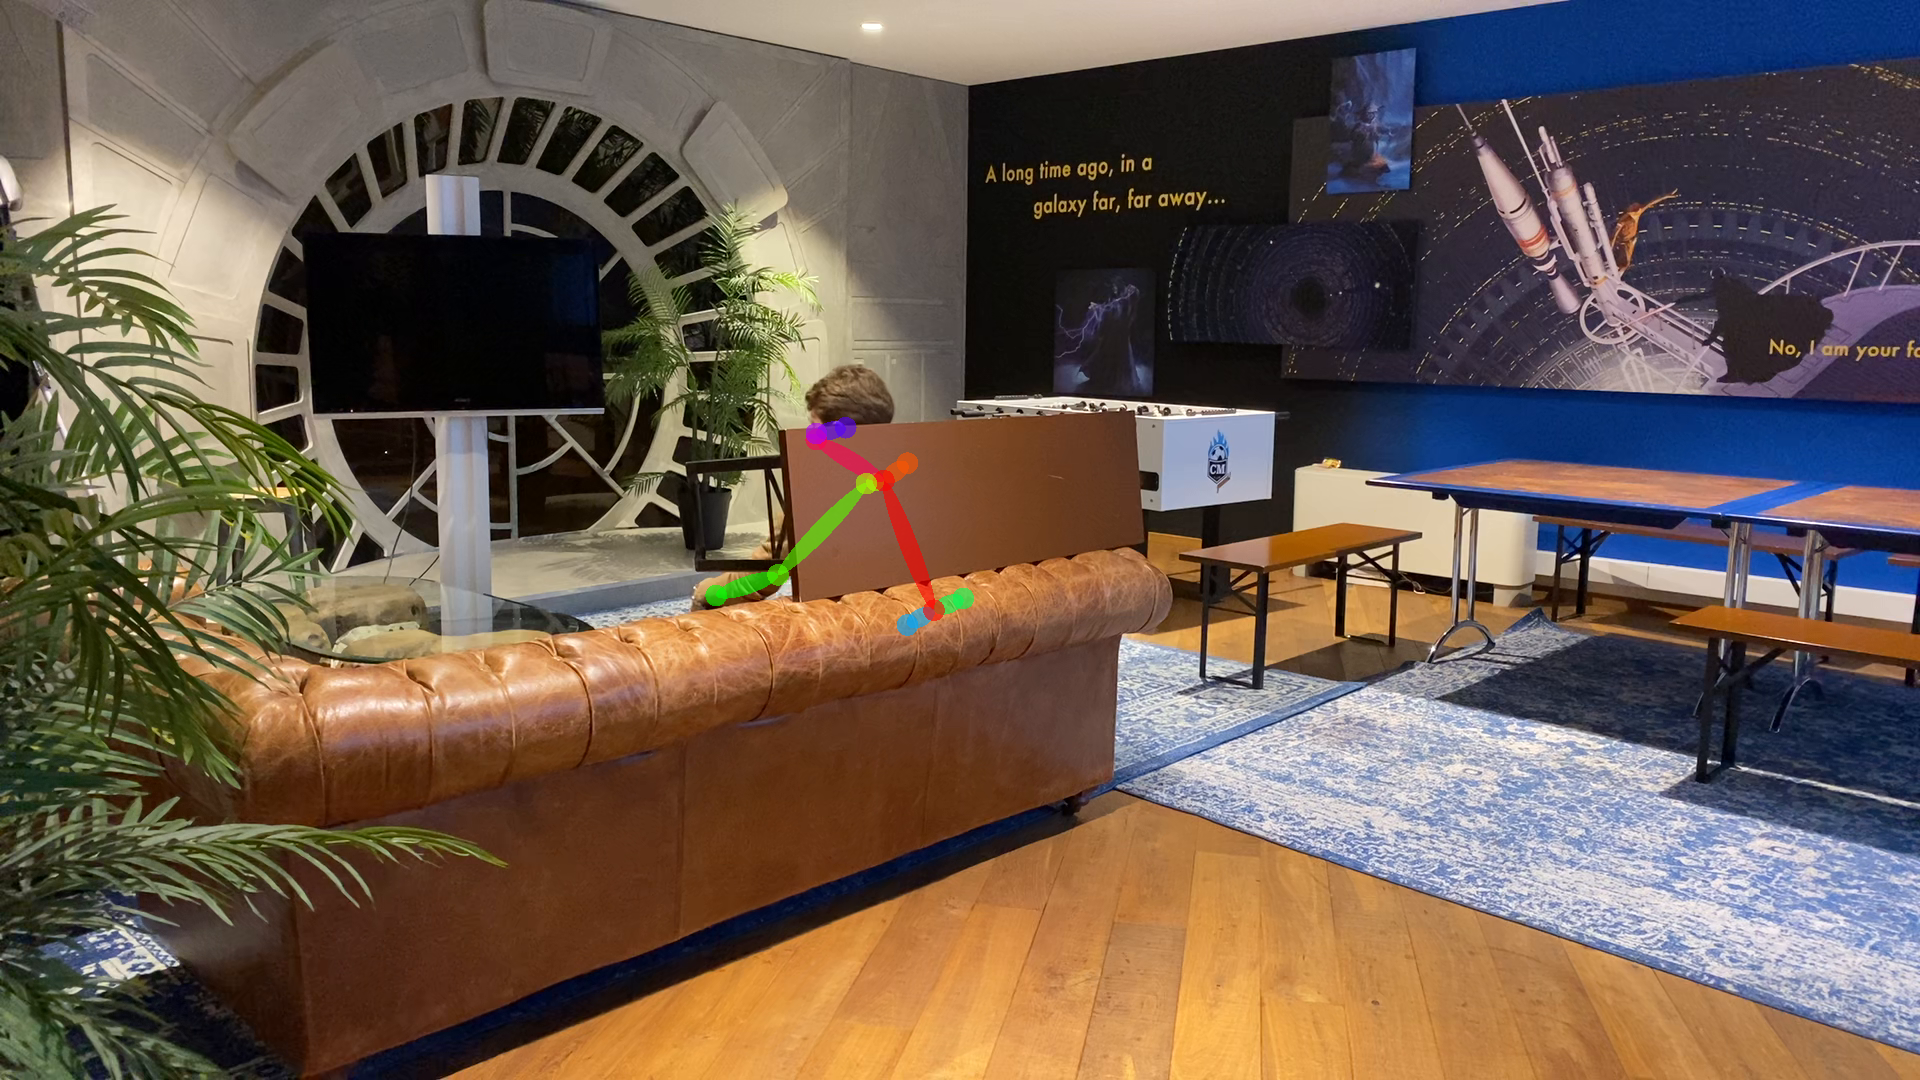
\includegraphics[width=0.3\textwidth]{Figures/humor/qualitative/good/sitting/openPose.png}} 
    \hfil
    \subfloat[Stage 2]{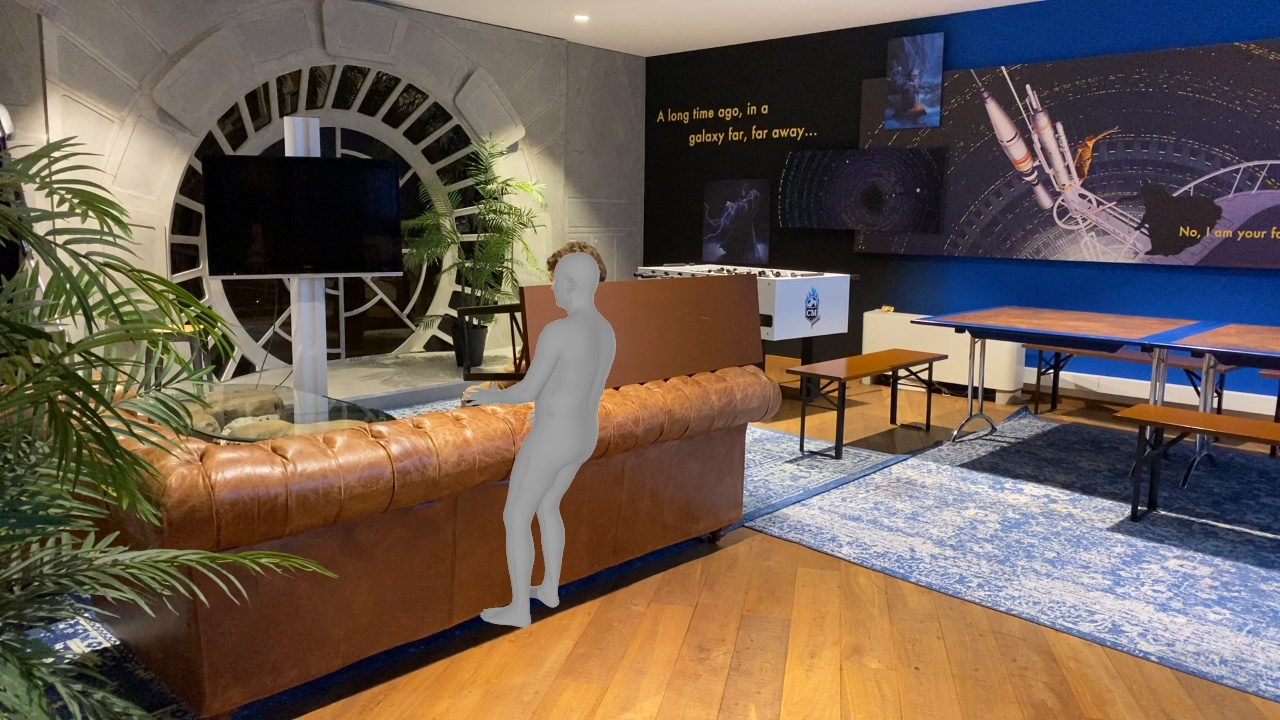
\includegraphics[width=0.3\textwidth]{Figures/humor/qualitative/good/sitting/stage2.jpg}} 
    \hfil
    \subfloat[Stage 3]{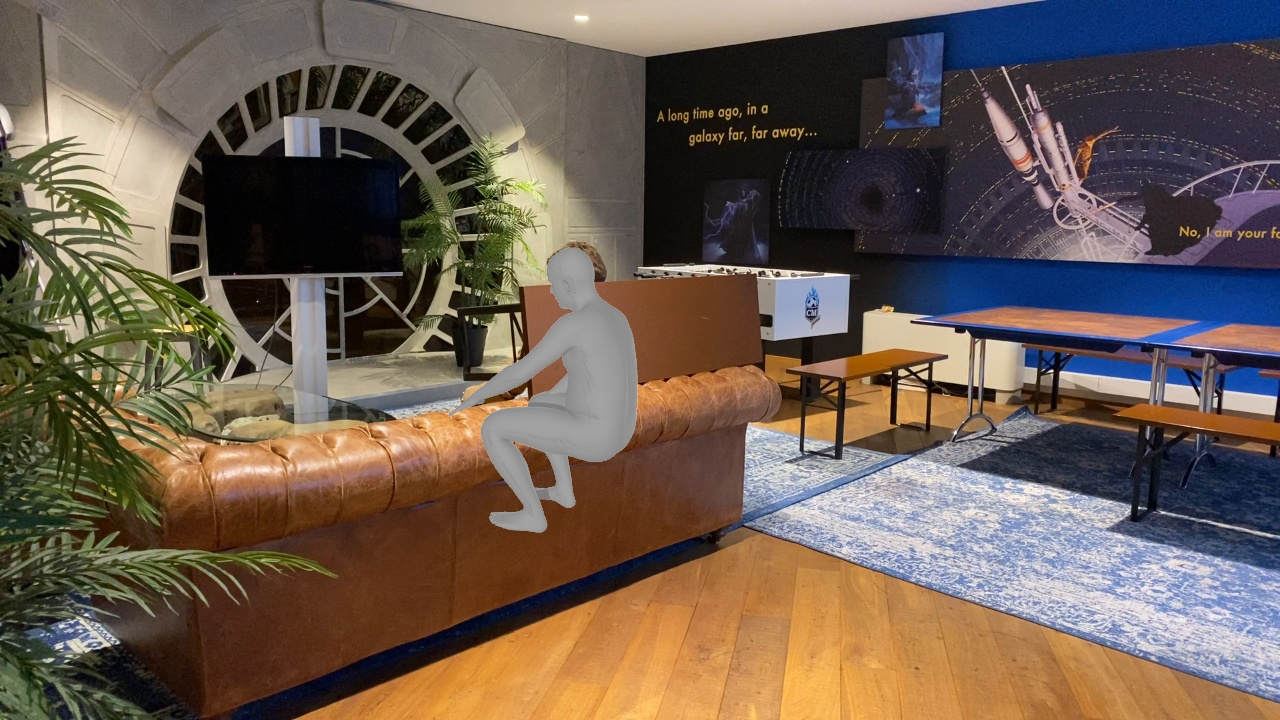
\includegraphics[width=0.3\textwidth]{Figures/humor/qualitative/good/sitting/stage3.jpg}}
    \caption{HuMoR achieving occluded sitting}
    \label{fig:humor_sitting}
\end{figure}

We also note in many of the less difficult videos, that HuMoR produces clean motion and deals with many abnormal movements without obvious issues. It therefore doesn't seem to regress the easy situations, but can improve the more difficult situations, notably occlusions.


\subsection{Drawbacks of HuMoR}

We noted that while HuMoR manages to sit when occluded, it often fails to walk. This seems to be due to the fact that OpenPose often predicts both legs on the frames just before the occlusions where only one leg is actually un-occluded, as can be seen in \figref{fig:humor_bad_occluded_walking}. This results in a sequence of poses where the frames before an occlusion indicate that the person is no longer walking, hence making it significantly more difficult for HuMoR to begin walking again during the occlusion. This issue is thus probably largely due to HuMoRs' TestOps' dependence on OpenPose and thus it's inheritence of OpenPoses' failure points.

\begin{figure}[!ht]
    \centering
    \subfloat[OpenPose]{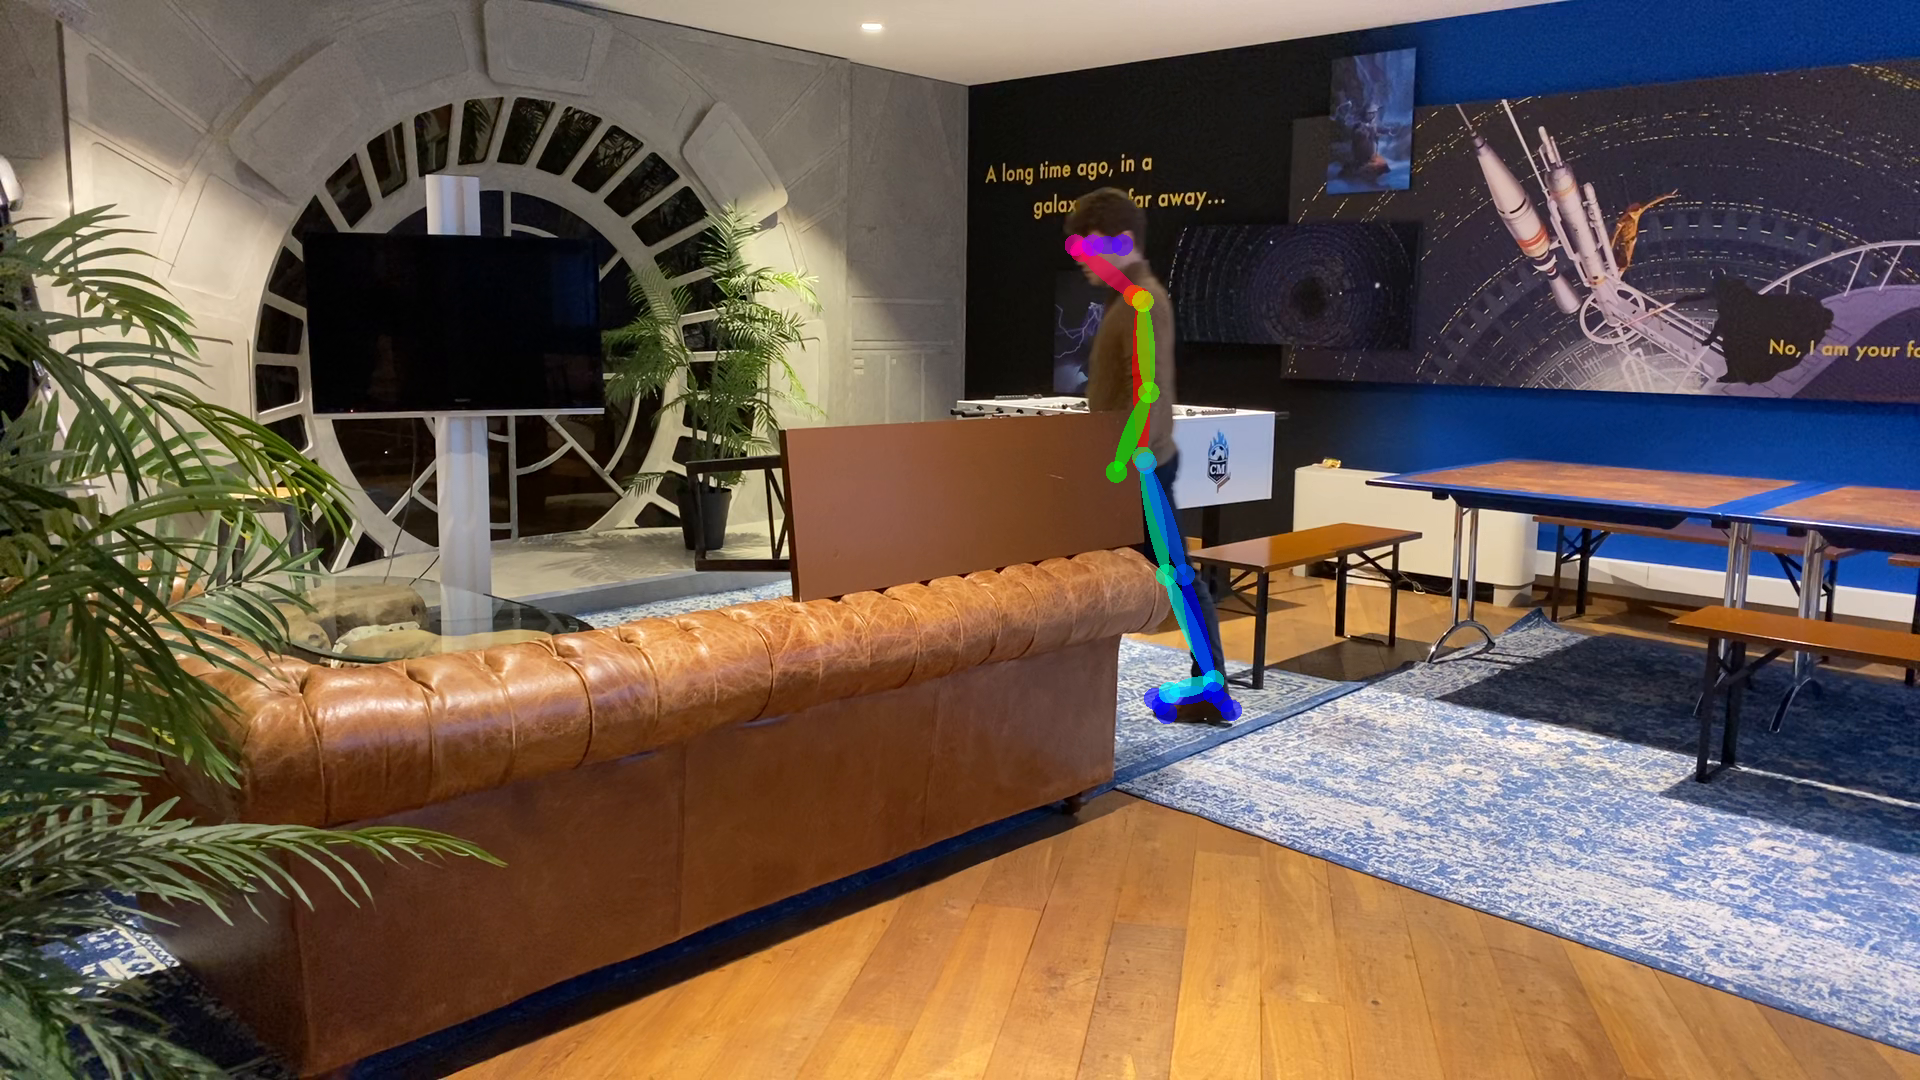
\includegraphics[width=0.3\textwidth]{Figures/humor/qualitative/bad/occluded_walking_failed/openPose.png}} 
    \hfil
    \subfloat[Stage 2]{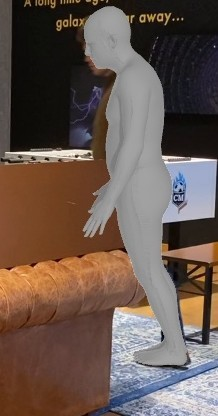
\includegraphics[width=0.3\textwidth]{Figures/humor/qualitative/bad/occluded_walking_failed/stage2.jpg}} 
    \hfil
    \subfloat[Stage 3]{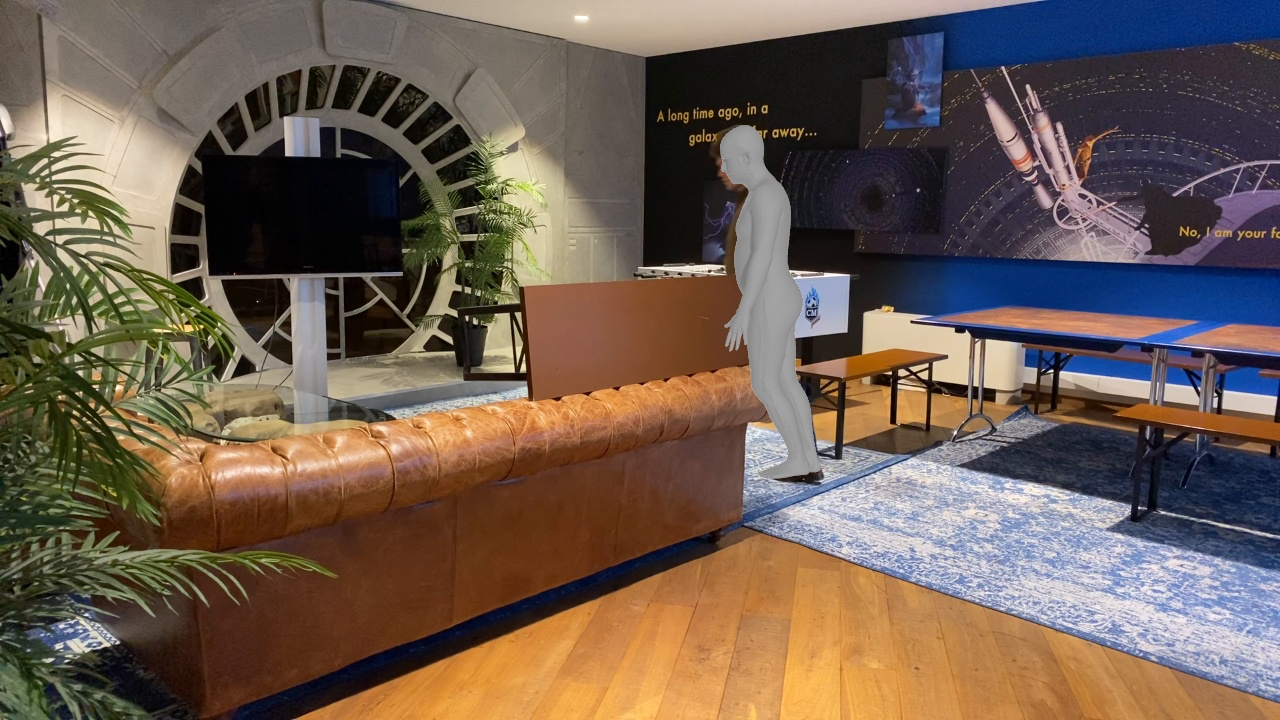
\includegraphics[width=0.3\textwidth]{Figures/humor/qualitative/bad/occluded_walking_failed/stage3.jpg}}
    \caption{Occluded walking failure point, 2 legs predicted instead of 1}
    \label{fig:humor_bad_occluded_walking}
\end{figure}

We also found that the choice of axis angle representation for various rotations led to the emergence of common known issue that arising from the discontinuities present in the representation \cite{aa_6d_angles}. The shortest path between certain angles in axis angle space can lead to a 360 degree rotation, as seen in \figref{fig:humor_bad_aa}, among other issues.

\begin{figure}[!ht]
    \centering
    \subfloat[]{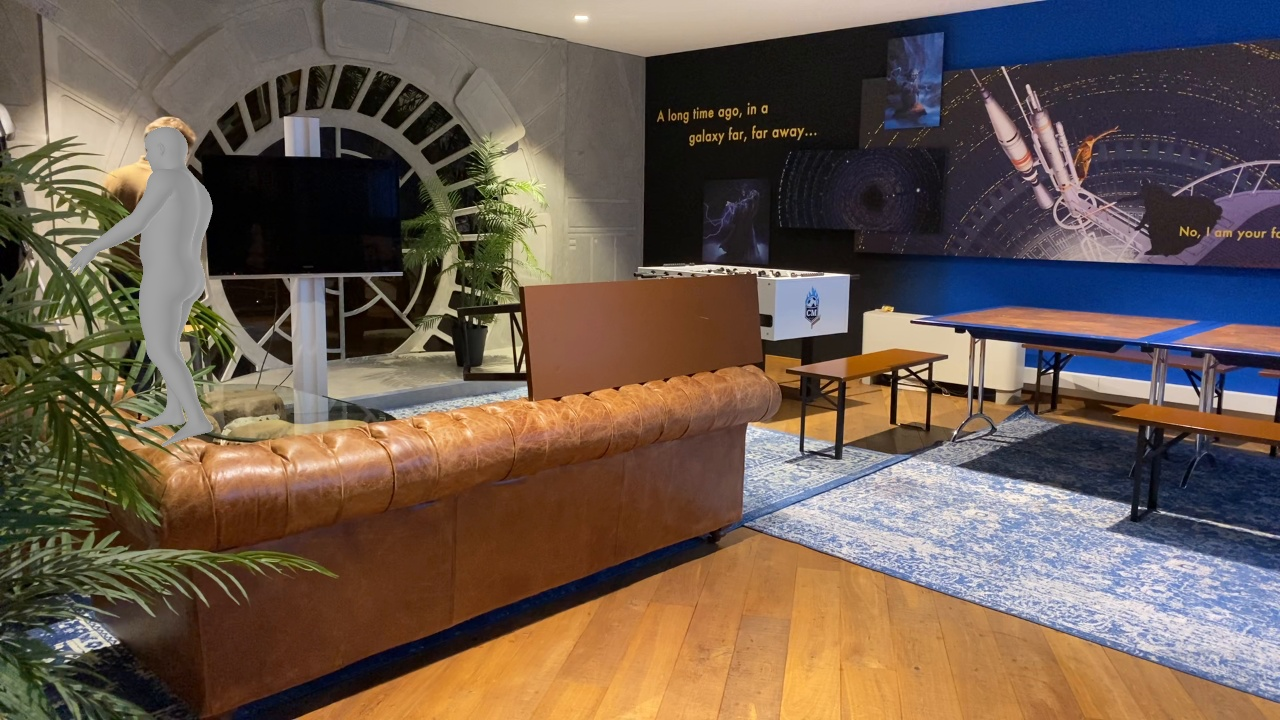
\includegraphics[width=0.3\textwidth]{Figures/humor/qualitative/bad/aa_issue/frame_00000331.jpg}}
    \hfil
    \subfloat[]{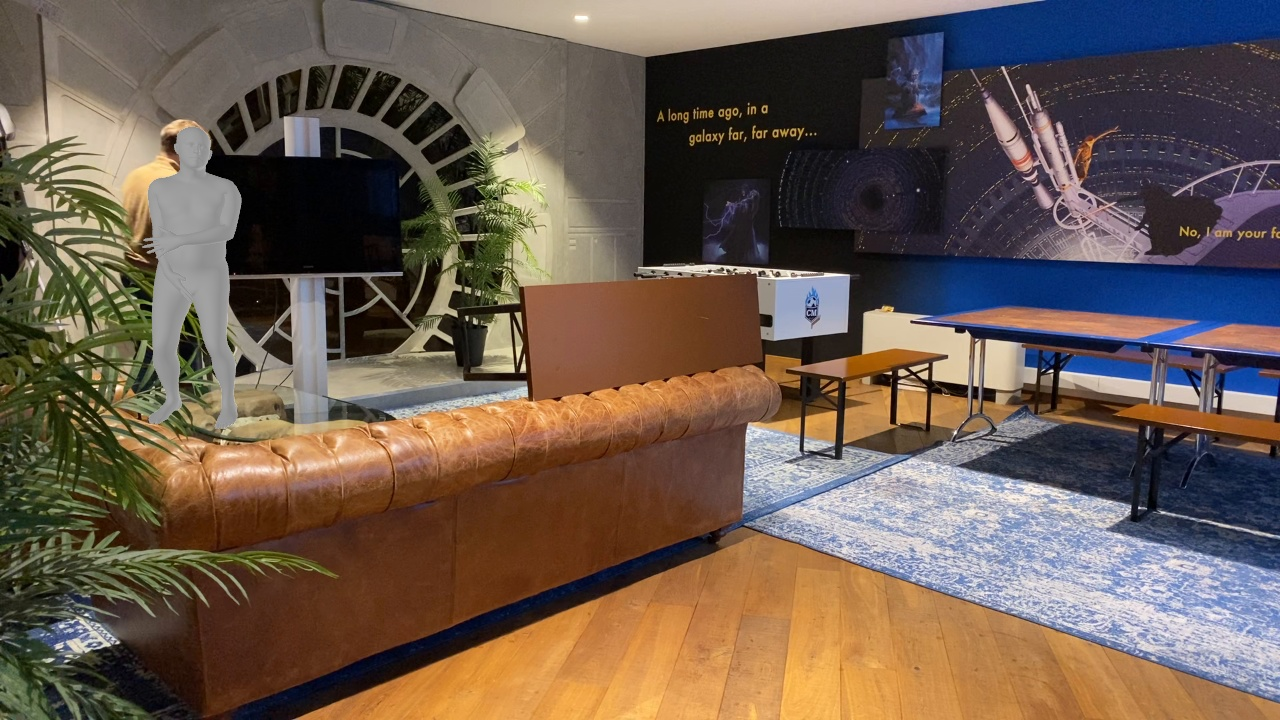
\includegraphics[width=0.3\textwidth]{Figures/humor/qualitative/bad/aa_issue/frame_00000336.jpg}} 
    \hfil
    \subfloat[]{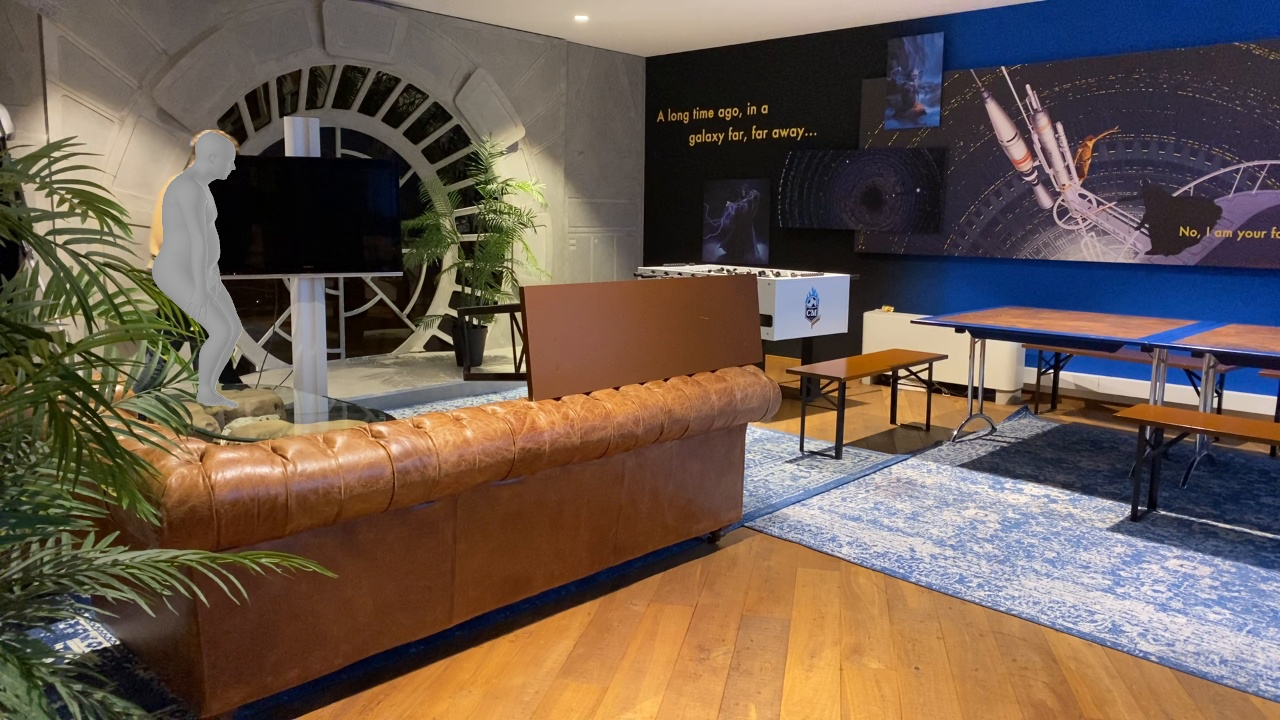
\includegraphics[width=0.3\textwidth]{Figures/humor/qualitative/bad/aa_issue/frame_00000342.jpg}}
    \caption{Axis angle issue: dubious rotations}
    \label{fig:humor_bad_aa}
\end{figure}

We found that the TestOps system would occasionally get itself into a tangle, as seen in \figref{fig:humor_bad_mess}, we assume due to the autogregressive nature resulting in a potentially catastrophic cumulation of errors, and found this happended most notably for a sequence containing someone rolling on the floor. It is interesting to note that these sorts of motions were not often, if ever, present in the training data.

\begin{figure}[!ht]
    \centering
    \subfloat[OpenPose]{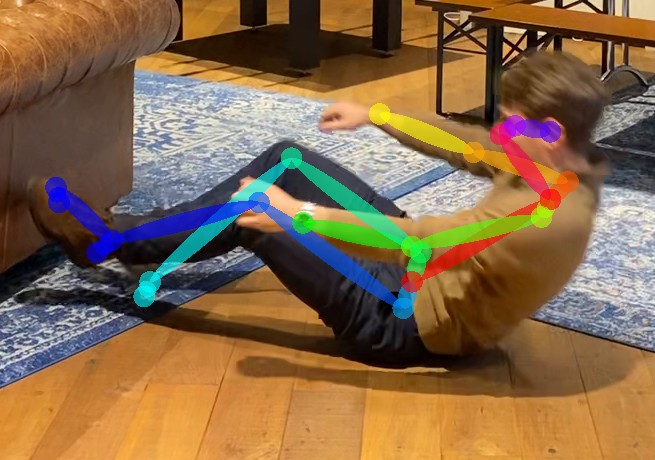
\includegraphics[width=0.3\textwidth]{Figures/humor/qualitative/bad/unrecoverable/openPose.png}} 
    \hfil
    \subfloat[Stage 2]{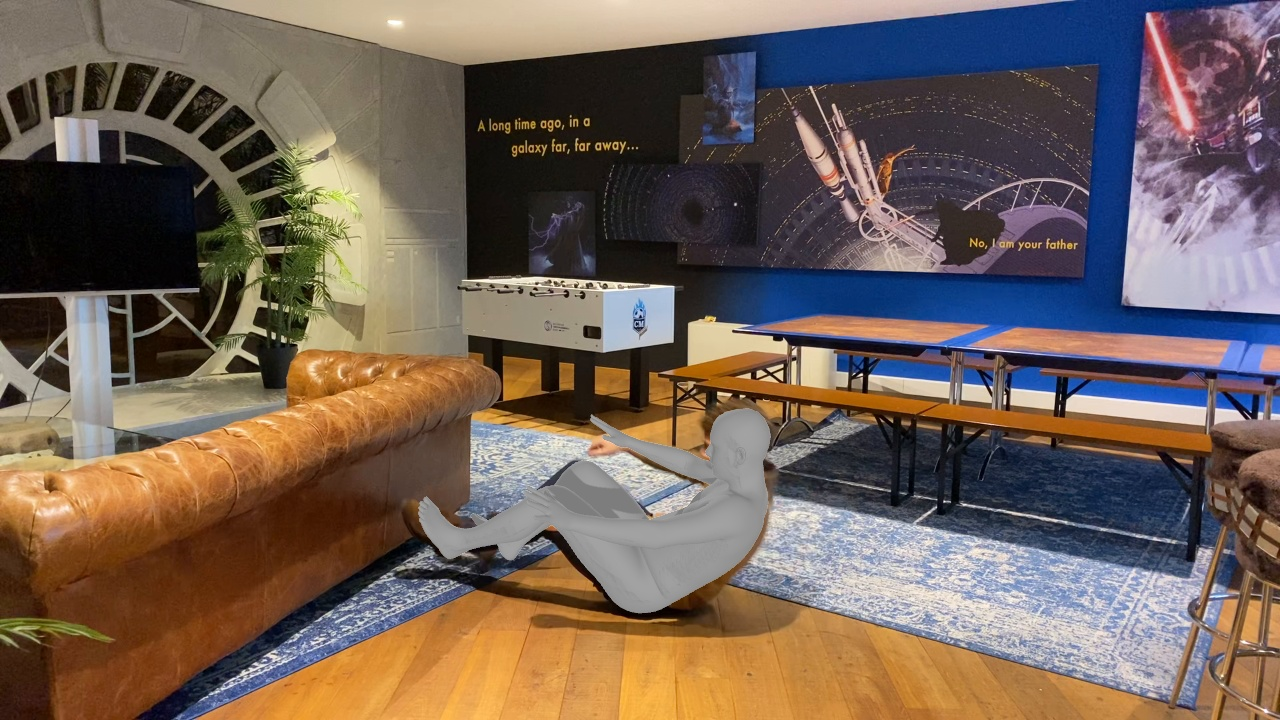
\includegraphics[width=0.3\textwidth]{Figures/humor/qualitative/bad/unrecoverable/stage2.jpg}} 
    \hfil
    \subfloat[Stage 3]{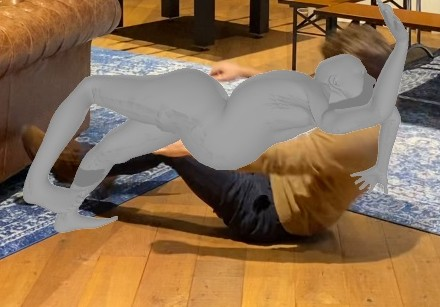
\includegraphics[width=0.3\textwidth]{Figures/humor/qualitative/bad/unrecoverable/stage3.jpg}}
    \caption{HuMoR in a tangle}
    \label{fig:humor_bad_mess}
\end{figure}

Next, we saw overly smoothed motion for certain clips, most notably for particularly stylised motion such as dancing.  We also found that if there is a single frame without Open Pose predictions then as of that frame the TestOps fails. Finally, and most importantly, we found that the TestOps was extremely slow. It took around 20mins per 2s clip, and that we could batch at most 4 2s clips together, so 20mins per 8s on a Nvidia GeoForce 1080ti with 11Gbs memory.

We concluded that there were a number of potential benifits, notably in occluded situations, and that many of the issues, including the axis angle representation issue, the dependence on humor, and smooth motion, have a good chance of being fixed with different design choices.  The glaring issue however was the unresonable amount of time the system took, rendering it unusable for our purposes as we wish the system to be close to real time.

\subsection{Profiling}
To investigate this speed issue, we profiled the code, as can be seen in \figref{fig:humor_profiling}. We found that the program spent 90\% of it's time in the Stage 3 optimiser closure, 56\% of it's time performing the backwards step and 32\% of it's time in the rollout function. Hence it was clear that the speed issue was due to the slow act of rolling out and the large computation necessary to perform the backwards step on the large computation graph resulting from the rollout.

\begin{figure}[!ht]
    \centering
    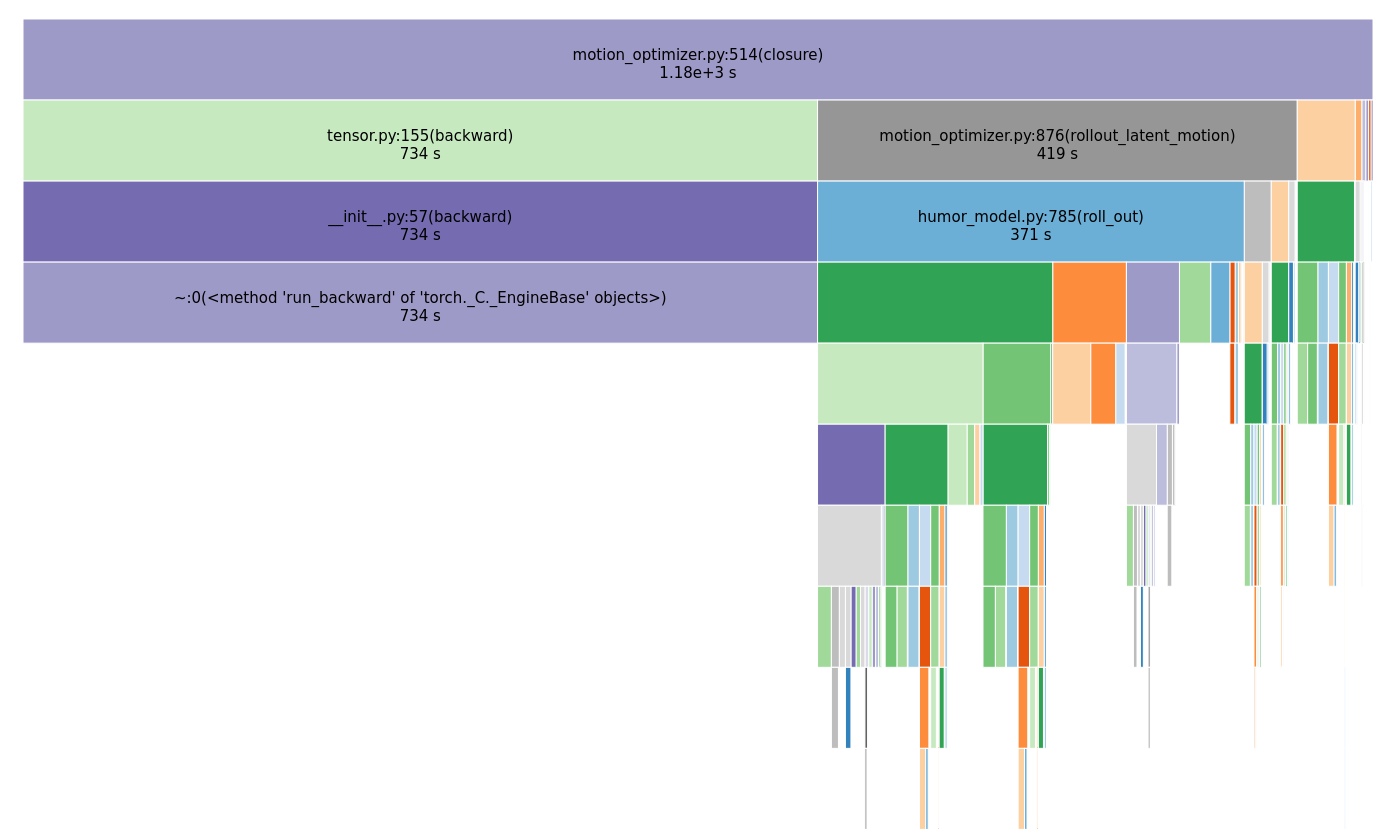
\includegraphics[width=1\textwidth]{Figures/humor/profiling/profiling.png}
    \caption{TestOps profiling}
    \label{fig:humor_profiling}
\end{figure}

\subsection{Conclusion}
We came to the final conclusion that the HuMoR motion model alongside the TestOps optimisation showed potential, but that it must be sped up before we can conclusively say if it is of particular use to us. We note that to speedup the method, we must primarily focus on improving/removing the rollout. Thus, in the next section, an attempt to speed up the TestOps is made.
